\section{基本概念}

\begin{frame}\ft{常量}
\begin{dingyi}[常量]

在程序执行过程中,其值不发生改变的量称为常量。
\end{dingyi} \vspace{0.1in}

常量分为两类:\vspace{0.05in}

\begin{enumerate}
\item 直接常量(或字面常量)\\[0.1in]
\item 符号常量
\end{enumerate}
\end{frame}


\begin{frame}\ft{直接常量}

\begin{itemize}
\item 整型常量:\lstinline|12, 0, -3|;\\[0.1in]
\item 浮点型常量:\lstinline|3.1415, -1.23|;\\[0.1in]
\item 字符型常量:\lstinline|'a', 'b'|
\end{itemize}
\end{frame}

\begin{frame}[fragile]\ft{符号常量}

\begin{dingyi}[标识符]
用来标识变量名、符号常量名、函数名、数组名、类型名、文件名的有效字符序列。
\end{dingyi} \pause \vspace{0.1in}

\begin{dingyi}[符号常量]

在C语言中,可以用一个标识符来表示一个常量,称之为符号常量。
\end{dingyi} 
\end{frame}

\begin{frame}[fragile]\ft{符号常量}
符号常量在使用之前必须先定义,其一般形式为:
\begin{lstlisting}
#define `标识符` `常量`
\end{lstlisting}
\vspace{0.05in}

\begin{itemize}
\item \lstinline|#define|是一条预处理命令,称为宏定义命令。\\[0.1in]
\item 功能是把该标识符定义为其后的常量值。\\[0.1in]
\item 一经定义,以后在程序中所有出现该标识符的地方均代之以该常量值。
\end{itemize}
\end{frame}

\begin{frame}[fragile]\ft{符号常量}
\begin{lstlisting}
#include<stdio.h>
#define PRICE 100
int main(void)
{
  int num, total;  
  num = 10;
  total = num * PRICE;
  printf("total=%d\n", total);  
  return 0;
}
\end{lstlisting}

\end{frame}

\begin{frame}[fragile]\ft{符号常量}
使用符号常量的好处是:\vspace{0.05in}

\begin{itemize}
\item 含义清楚;\\[0.1in]
\item 能做到“一改全改”。
\end{itemize}
\end{frame}


\begin{frame}\ft{变量}
\begin{dingyi}\red{变量}

在程序执行过程中,其值可以改变的量称为变量。
\end{dingyi}

\begin{itemize}
\item
一个变量应该有一个名字,在内存中占据一定的存储单元。\\[0.1in]
\item
变量定义必须放在变量使用之前。
\end{itemize}
\end{frame}


\begin{frame}\ft{变量}
\begin{itemize}
\item
一般放在函数体的开头部分。\\[0.1in]
\item
要区分变量名和变量值是两个不同的概念。
\end{itemize}

\begin{figure}
\centering
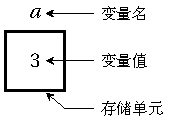
\includegraphics[width=3.5in]{ch03/images/var}
\end{figure}

\end{frame}


\begin{frame}\ft{数据类型}
\begin{figure}
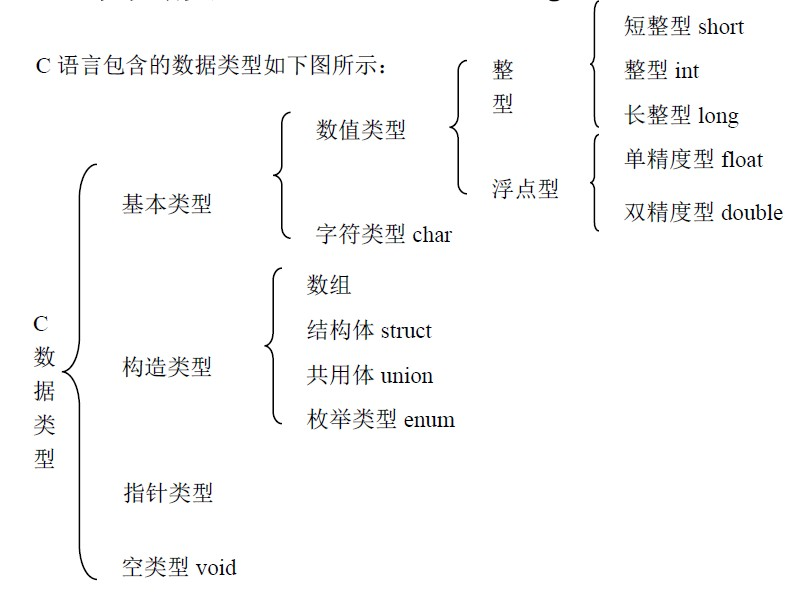
\includegraphics[width=3.5in]{ch03/images/datatype}
\end{figure}
\end{frame}


\begin{frame}\ft{数据类型}
\begin{itemize}
\item 
对于常量,编译器通过书写形式来辨认其类型。\\[0.1in]
\item[] 例如,\lstinline|42|是整型,\lstinline|42.0|是浮点型。\\[0.2in]
\item
变量必须在声明语句中指定其类型。
\end{itemize}
\end{frame}

\begin{frame}\ft{数据类型关键字}
\begin{table}
\centering
\begin{tabular}{p{3cm}|p{3cm}|p{3cm}}\hline
\lstinline|int| & \lstinline|signed| & \lstinline|_Bool| \\[0.05in]
\lstinline|long| & \lstinline|void| & \lstinline|_Complex| \\[0.05in]
\lstinline|short| & & \lstinline|_Imaginary|\\[0.05in]
\lstinline|unsigned| &&\\[0.05in]
\lstinline|char| &&\\[0.05in]
\lstinline|float| &&\\[0.05in]
\lstinline|double| &&\\\hline
\end{tabular}
\end{table}
\end{frame}

\begin{frame}[fragile]\ft{数据类型关键字}
\begin{itemize}
\item 
\lstinline|int|提供基本整型,\lstinline|long|、\lstinline|short|、\lstinline|unsigned|和\lstinline|signed|为其变种。\\[0.1in]
\item
\lstinline|char|用于表示字母及其他字符(如\lstinline|#, $, %,*|等),也可表示小的整数。\\[0.1in]
\item
\lstinline|float|、\lstinline|double|和\lstinline|long double|表示浮点型数。\\[0.1in]
\item \lstinline|_Bool|表示布尔值(\lstinline|true|和\lstinline|false|)。\\[0.1in]
\item \lstinline|_Complex|和\lstinline|_Imaginary|分别表示复数和虚数。\\[0.2in]
\end{itemize}
\red{这些类型按其存储方式被分为两类:整型和浮点型。}
\end{frame}





